\chapter{Vectores, rangos y más bucles}
\label{sec:vectores}
  
\section{Más bucles}

\lettrine[lines=2]{A}{ntonia aprobó} con una amplia sonrisa el trabajo de
Cecilia:

---Só\-lo para que lo tengas en cuenta ---aclaró---,
\openscad{} te permite declarar más de una variable en el mismo bucle;
por ejemplo, tu solución al cilindro puede escribirse también así:

  \begin{figure}[ht]
  \begin{minipage}[]{.5\textwidth}
    \begin{lstlisting}
$fn=200;

for(z=[0:5:30],
    x=[20:-5:0],
    alfa=[0:15:359])
   rotate([0,0,alfa])
    translate([x,0,z])
     sphere(r=2);
    \end{lstlisting}%$
  \end{minipage}\hfill
    \begin{minipage}[]{.5\textwidth}
      \centering
      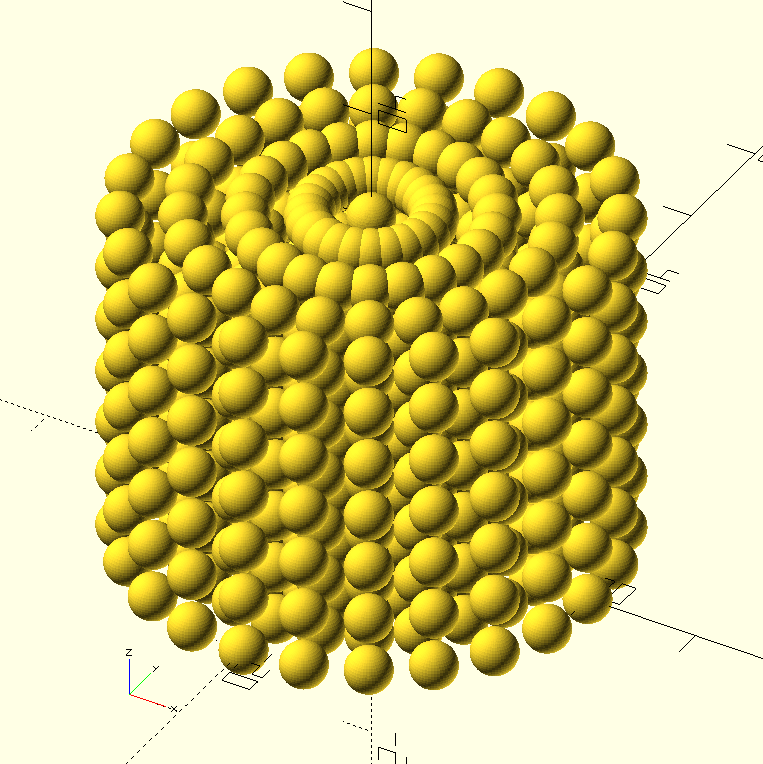
\includegraphics[width=.8\textwidth]{imagenes/cilindro-de-esferas}
    \end{minipage}
    \caption{Antonia declara un \lstinline!for! con más de una
      variable.}
      \label{fig:cilindro-de-esferas-10}
    \end{figure}


    Cecilia no estaba segura de que esta reescritura mejorara su
    texto, pero decidió que una nueva posibilidad expresiva siempre
    merecía ser tenida en cuenta.


  \section{Vectores}

  ---Un tipo de valor muy útil en \openscad{} es el denominado
  \emph{vector} ---dijo Antonia---, que no es otra cosa que una
  colección ordenada de otros valores. Se escribe encerrando estos
  entre corchetes y separados por comas; por ejemplo, el vector
  \lstinline![23,12,71]!  tiene tres elementos: el 23, el 12 y el 71.

  Cecilia reconoció de inmediato esa sintaxis:

  ---¡Estuvimos usando vectores todo el tiempo! En
  \lstinline!translate!, \lstinline!rotate! y para indicar el tamaño
  de un cubo, por ejemplo.

  ---Tal cual ---acordó Antonia---. Y ahora, sabiendo
    que los vectores no son otra cosa que valores particulares en sí
    mismos, podemos guardarlos en variables también:

  \begin{figure}[ht]    
  \begin{minipage}[]{.5\textwidth}
    \begin{lstlisting}
v = [10,20,30];

rotate(v)
  translate(v)
    cube(v);
\end{lstlisting}
  \end{minipage}\hfill
    \begin{minipage}[]{.5\textwidth}
      \centering
      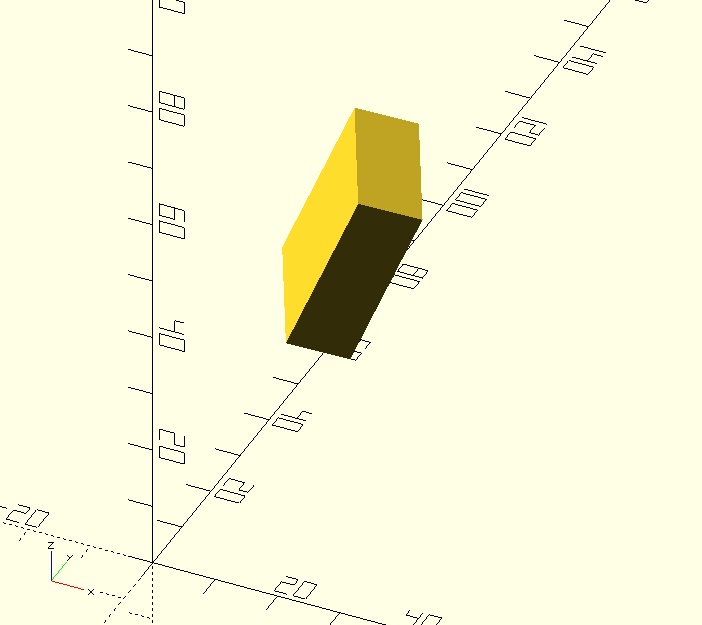
\includegraphics[width=.8\textwidth]{imagenes/cubo-v}
    \end{minipage}
    \caption{Antonia abusa de las posibilidades de los vectores.}
      \label{fig:abuso-de-vectores}
    \end{figure}


    A Cecilia el ejemplo le pareció muy tonto, pero captó la idea.

  Antonia prosiguió:

  ---Es importante que tengas en cuenta que entre los valores que un
  vector admite se encuentran, también, los propios vectores; es decir, podemos tener
  vectores de vectores. En ese caso solemos hablar de
  \emph{matrices}. Nos resultarán utilísimas cuando escribamos nuestro
  reloj de Sol digital. Un ejemplo posible es \lstinline![[1,2,3],[4,5,6],[7,8,9]]!, vector cuyos elementos son los vectores \lstinline![1,2,3]!, \lstinline![4,5,6]! y \lstinline![7,8,9]!.

  \begin{figure}[ht]    
  \begin{minipage}[]{.6\textwidth}
    \begin{lstlisting}
v = [[10,20,30],
     [40,-10,-15],
     [0,-90,0]];
rotate(v[2])
  translate(v[1])
    cube(v[0]);
// Lo anterior es
// equivalente a:    
//rotate([0,-90,0])
// translate([40,-10,-15])
//  cube([10,20,30]);
\end{lstlisting}
  \end{minipage}\hfill
    \begin{minipage}[]{.4\textwidth}
      \centering
      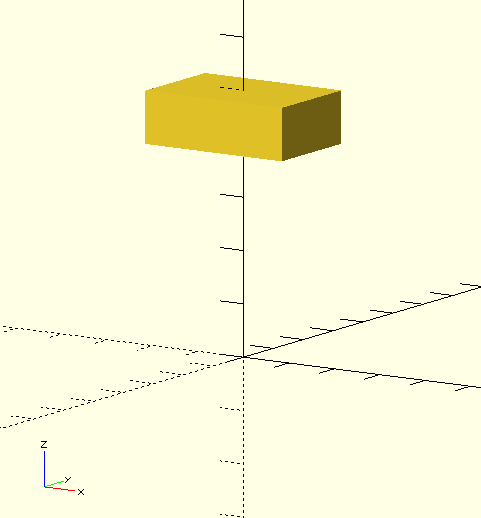
\includegraphics[width=\textwidth]{imagenes/cubo-vector}
    \end{minipage}
    \caption{Antonia usa un vector de vectores (también conocido como
      matriz) y se refiere a sus elementos mediante índices.}
      \label{fig:matrices-1}
    \end{figure}

  
  \guillemotright En un vector es importante el orden de los elementos
  ---continuó Antonia---: cada uno tiene su posición
  particular. Decimos que el primero está en la posición `0', el
  segundo en la posición `1', y así siguiendo. La razón de comenzar en
  `0' tiene que ver con la manera en que almacenan los números las
  computadoras; comenzar en `1' supondría desperdiciar memoria. En
  fin, es muy técnico ---concluyó Antonia agitando suavemente en el
  aire la mano derecha, como si el conjuro ``es muy técnico'' bastara
  para dar algo por explicado.

  \guillemotright Es posible referirse a un elemento en particular de
  un vector adosándole, al final, el apéndice \lstinline![i]!, donde
  \lstinline!i! representa la posición del elemento de nuestro
  interés. Así, \lstinline![4,5,6][0]! es el elemento \lstinline!4!,
  \lstinline![[1,2,3],[4,5,6],[7,8,9]][1]!  vale tanto como
  \lstinline![4,5,6]!, etc. A ver si con el ejemplo de la figura
  \ref{fig:matrices-1} queda más claro.  Como comentario en las líneas
  7 a 11 te puse un código equivalente al escrito en las líneas 1 a
  6.

  Cecilia seguía sintiendo que se trataba de un ejemplo muy tonto,
  pero se conformó con entender el punto.


  \section{Rangos}

  ---Los rangos que venimos utilizando en los bucles podrían ser
  contemplados como vectores `comprimidos'; quiero decir, a una le
  gustaría pensar que algo como \lstinline![0:2:10]! equivale al
  vector \lstinline![0,2,4,6,8,10]! ---Antonia seguía disertando, con
  su molesto tono didáctico---. Pero la semejanza es superficial; por
  ejemplo, escribir algo como \lstinline![0:2:10][3]!, en lugar de
  devolvernos el valor 6, nos tira un error. Lo que sí admiten los
  rangos es ser aludidos mediante una variable; así, es posible
  escribir un cubo de esferas de esta limpia manera ---agregó,
  señalando la figura \ref{fig:rangos-1}.

  \begin{figure}[ht]    
  \begin{minipage}[]{.5\textwidth}
    \begin{lstlisting}
$fn= 50;

s = [0:10:100];

for(x=s,y=s,z=s)
  translate([x,y,z])
    sphere(2);
\end{lstlisting}%$
  \end{minipage}\hfill
    \begin{minipage}[]{.5\textwidth}
      \centering
      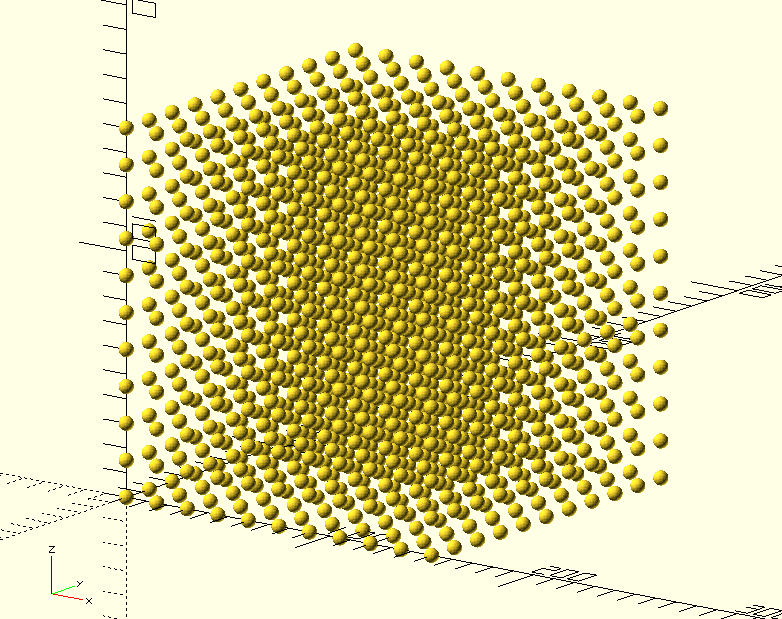
\includegraphics[width=.8\textwidth]{imagenes/cubo-de-esferas}
    \end{minipage}
    \caption{Antonia asigna un rango a una variable a modo de
      ejemplo.}
      \label{fig:rangos-1}
    \end{figure}


    Este texto a Cecilia le gustó un poco más; comprendió que, en el
    fondo, era equivalente al de la figura \ref{fig:rangos-2}. La
    diferencia entre ambos era que si una quería modificar el tamaño
    del cubo, en el primer caso bastaba con cambiar el valor de la
    variable \texttt{s} en la línea 3, mientras que en el segundo era
    preciso modificar las líneas 3 a 5.

  
  \begin{figure}[ht]    
  \begin{minipage}[]{.5\textwidth}
    \begin{lstlisting}
$fn= 50;

for(x=[0:10:100],
    y=[0:10:100],
    z=[0:10:100])
  translate([x,y,z])
    sphere(2);
\end{lstlisting}%$
  \end{minipage}\hfill
     \begin{minipage}[]{.5\textwidth}
       \centering
       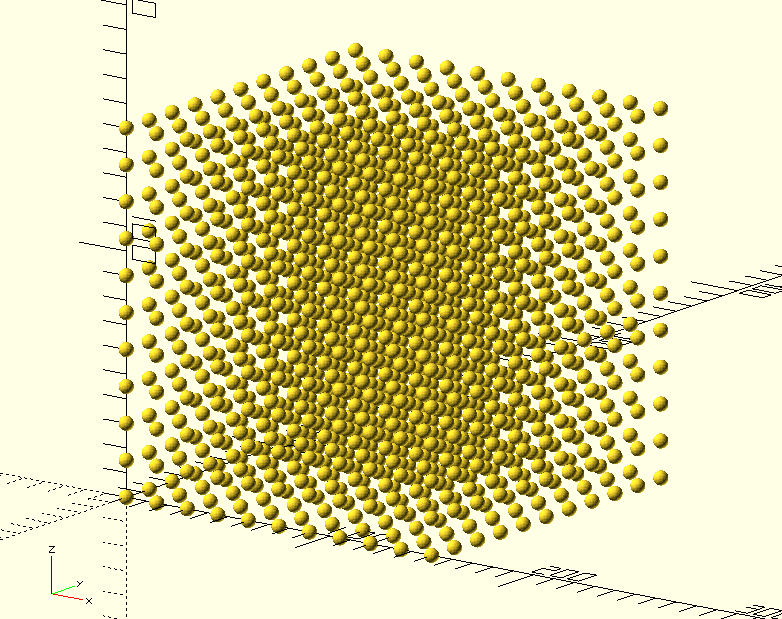
\includegraphics[width=.8\textwidth]{imagenes/cubo-de-esferas}
     \end{minipage}
     \caption{Cecilia desarrolla el ejemplo anterior de Antonia, para
       asegurarse de haber entendido el concepto.}
      \label{fig:rangos-2}
    \end{figure}



De todos modos, no pudo evitar considerar que, en ejemplos tan
minúsculos como estos, las diferencias terminaban diluyéndose en una
cuestión de gustos. Pero en todo caso le parecía que siempre resultaba
útil contar con más de una forma de escribir lo mismo: una nunca sabía
con qué problemas se enfrentaría más tarde, y disponer de un mayor
número de herramientas lingüísticas siempre era mejor.


%%% Local Variables:
%%% mode: latex
%%% TeX-master: "../libro"
%%% End:
